\section{Hadoop MapReduce to Spark}
\label{sec:history}
In several Big Data mining tools that have been developed, the most notable ones are MapReduce and Spark. MapReduce is a cluster computing framework 
which supports locality-aware scheduling, fault tolerance, and load balancing. Spark is designed to improve performance for iterative jobs keeping features of MapReduce. 

MapReduce provides a programming model where the user creates acyclic data flow graphs to pass input data through a set of operations. This 
data flow programming model is useful for many of query applications. However, MapReduce framework struggles from two of main resent data mining jobs: iterative jobs and interactive analysis. 

Iterative job is especially common in Machine Learning Algorithm, such as learning a data model using Gradient Descent. In traditional MapReduce framework, each iteration can be expressed as single MapReduce job 
so that each job must reload the data from disk. This leads I/O overhead and deteriorates performance of iterative algorithms. 

Interactive analysis is also an inevitable task in modern data science. A data scientist wants tp perform exploratory analysis in interactive way. 
Nevertheless, MapReduce is designed in the way more stable for ad-hoc query, so each analysis can be single MapReduce job. 
To perform multiple analysis to explore dataset, the data needs to be written to and reload from disk many times. 

To overcome these limitations, Spark has been developed as a new cluster computing framework maintaining the innovative characteristics of MapReduce and improving 
its iterative and interactive jobs with in-memory data structure.

Some of the notable improvements are shown here\cite{DBLP:journals/pvldb/ShiQMJWRO15}. For aggregation operation, map output selectivity, which is the ration of the map output size to the job input size, 
can be significantly reduced by using Spark. Spark uses a map side combiner, hash-based aggregation which is more efficient than sort-based aggregation used in MapReduce. 
For iterative operation, caching the input as Resilient Distributed Datasets (RDDs) can reduce CRU and disk I/O overheads for sequence iteration. 
This RDD caching takes a significant role to improve iterative job, because it is more efficient than other low-level caching approaches such as OS buffer caches, and HDFS caching. 
These caching strategy reduces disk I/O overhead, but CPU overhead, such as parsing text to objects.


\section{Apache Spark}
\label{sec:history}
\subsection{Resilient Distributed Datasets}
Major methods in Spark are Resilient Distributed Datasets (RDDs), a data structure that abstracts distributed memory across different clusters. 
The immutable coarse-grained transformation, spark-scheduler with lazy-evaluation, and memory management with cacheing achieve computation with fault-tolerance, 
fast execution, and moderate control on memory efficiency \cite{DBLP:conf/nsdi/ZahariaCDDMMFSS12}.

A RDD is essentially a multi-layer Java data structure. A top RDD object references Java array, which intern, references a set of tuple objects. 
The coarse-grained transformations and immutability requires a RDD to be deep-copied to produce a new RDD, but efficiently offers fault tolerance. 
The lost partitions of a RDD can be recomputed in parallel on different nodes rather than rolling back the whole program.

Spark-pipeline consists of sequence of transformations and actions over RDDs. A transformation produces a new RDD from a set of existing RDD. 
An action is method that computes statistics from an RDD. Due to lazy-evaluation nature, transformations do not materialize the newly created RDD. 
Instead, RDD Lineages are created. Lineage is a graph among parent and child RDDs which represents logical execution plan. 
This enhance fault-tolerance and improve ability to optimize execution plan. 

RDDs can be cached in memory for faster access by persist method. Developers can specify a storage level for a persisted RDD, in memory with serialized or deserialized, or on disk. 
Other than persisted RDD, Spark generates a lot of intermediate RDDs during execution. Since RDD is a Java object, they are managed by Garbage Collection (GC) in the JVM. 
However, persisted RDDs are never collected by GC. This GC might cause significant deterioration of performance of Spark, because GC shows heavy overhead when there are a number of objects.


\subsection{Memory Management in Spark}
Spark framework allocates multiple executors, JVMs, that run sequence of transformations and actions. As we describe the previous section, data in Spark is mainly stored as Java objects in memory, 
so that they are allocated on JVM heap and managed by JVM Garbage Collection. The data may form three types \cite{DBLP:journals/pvldb/XuGDWW19}: Cached data, Shuffled data, and Operator-generated data. 

Spark can cache data in memory to reduce disk I/O. This Cached data usually long-lived Java objects and span multiple stages in Spark-pipeline. 
Spark allocates a logical storage space to store the cached data as shown in Figure. After aggregation, Spark generates Shuffled data. Shuffled data is usually long-lived, 
because it need to be kept in memory until the task ends. Spark allocates execution space to store Shuffled data.
The storage space and execution space spans 60 \% of JVM heap space in default. Operator-generated data is data generated by user-defined operations. Since Operator-generated data may or may not be used, 
after the operation finish, the data object can be both short-lived or long-lived objects. These are stored in user space allocated on default 40 \% of JVM heap.

All data of these types on JVM heap is managed by JVM GC. GC check references graph of objects, mark whether the objects are used and deallocate memory space occupied by unused objects. 
There are three popular GCs: Parallel, CMS and G1. All of these method track generation of object based on the region of memory. 
The Java logical heap structure is shown in Figure~\ref{fig:javaheap}. As the figure shows, Java logical heap can be separated into three main parts where store objects for each corresponding generation: 
permanent generation, young generation, and old generation. The region for permanent generation stores metadata required by JVM to describe 
class and method used in application which will be permanently lived on the region of memory. The overview of Java GC is shown in Figure~\ref{fig:javagc}. 
The outer box represents region for particular generation. The inner box and the number represents object and its age in GC. 

The region for young generation mainly consists of two parts: Eden and Survivor space. 
First, Java objects are created in Eden space and promoted to Survivor space when survive from GC. 
After objects survive several GCs in Survivor space, they are finally promoted to old generation.

In region of old generation, JVM lunches multi-thread to perform GC. GC with multi-threading suffers from Stop-The-World (STW) pauses; 
GC may suspend application threads while performing object marking and deallocation. 
Different GC algorithms try to solve this problem with trade-off between GC frequency and memory utilization. 

Because of the problem of STW and copying objects to different physical memory pages , JVM GC cause huge overhead when number of objects is large. 
Therefore, GC become severe issue in Big Data processing where might produce significant number of object.

\begin{figure}[htb]
    \includegraphics[width=15cm]{java_heap.eps}
    \caption{Java Heap Structure}
    \label{fig:javaheap}
\end{figure}

\begin{figure}[htb]
    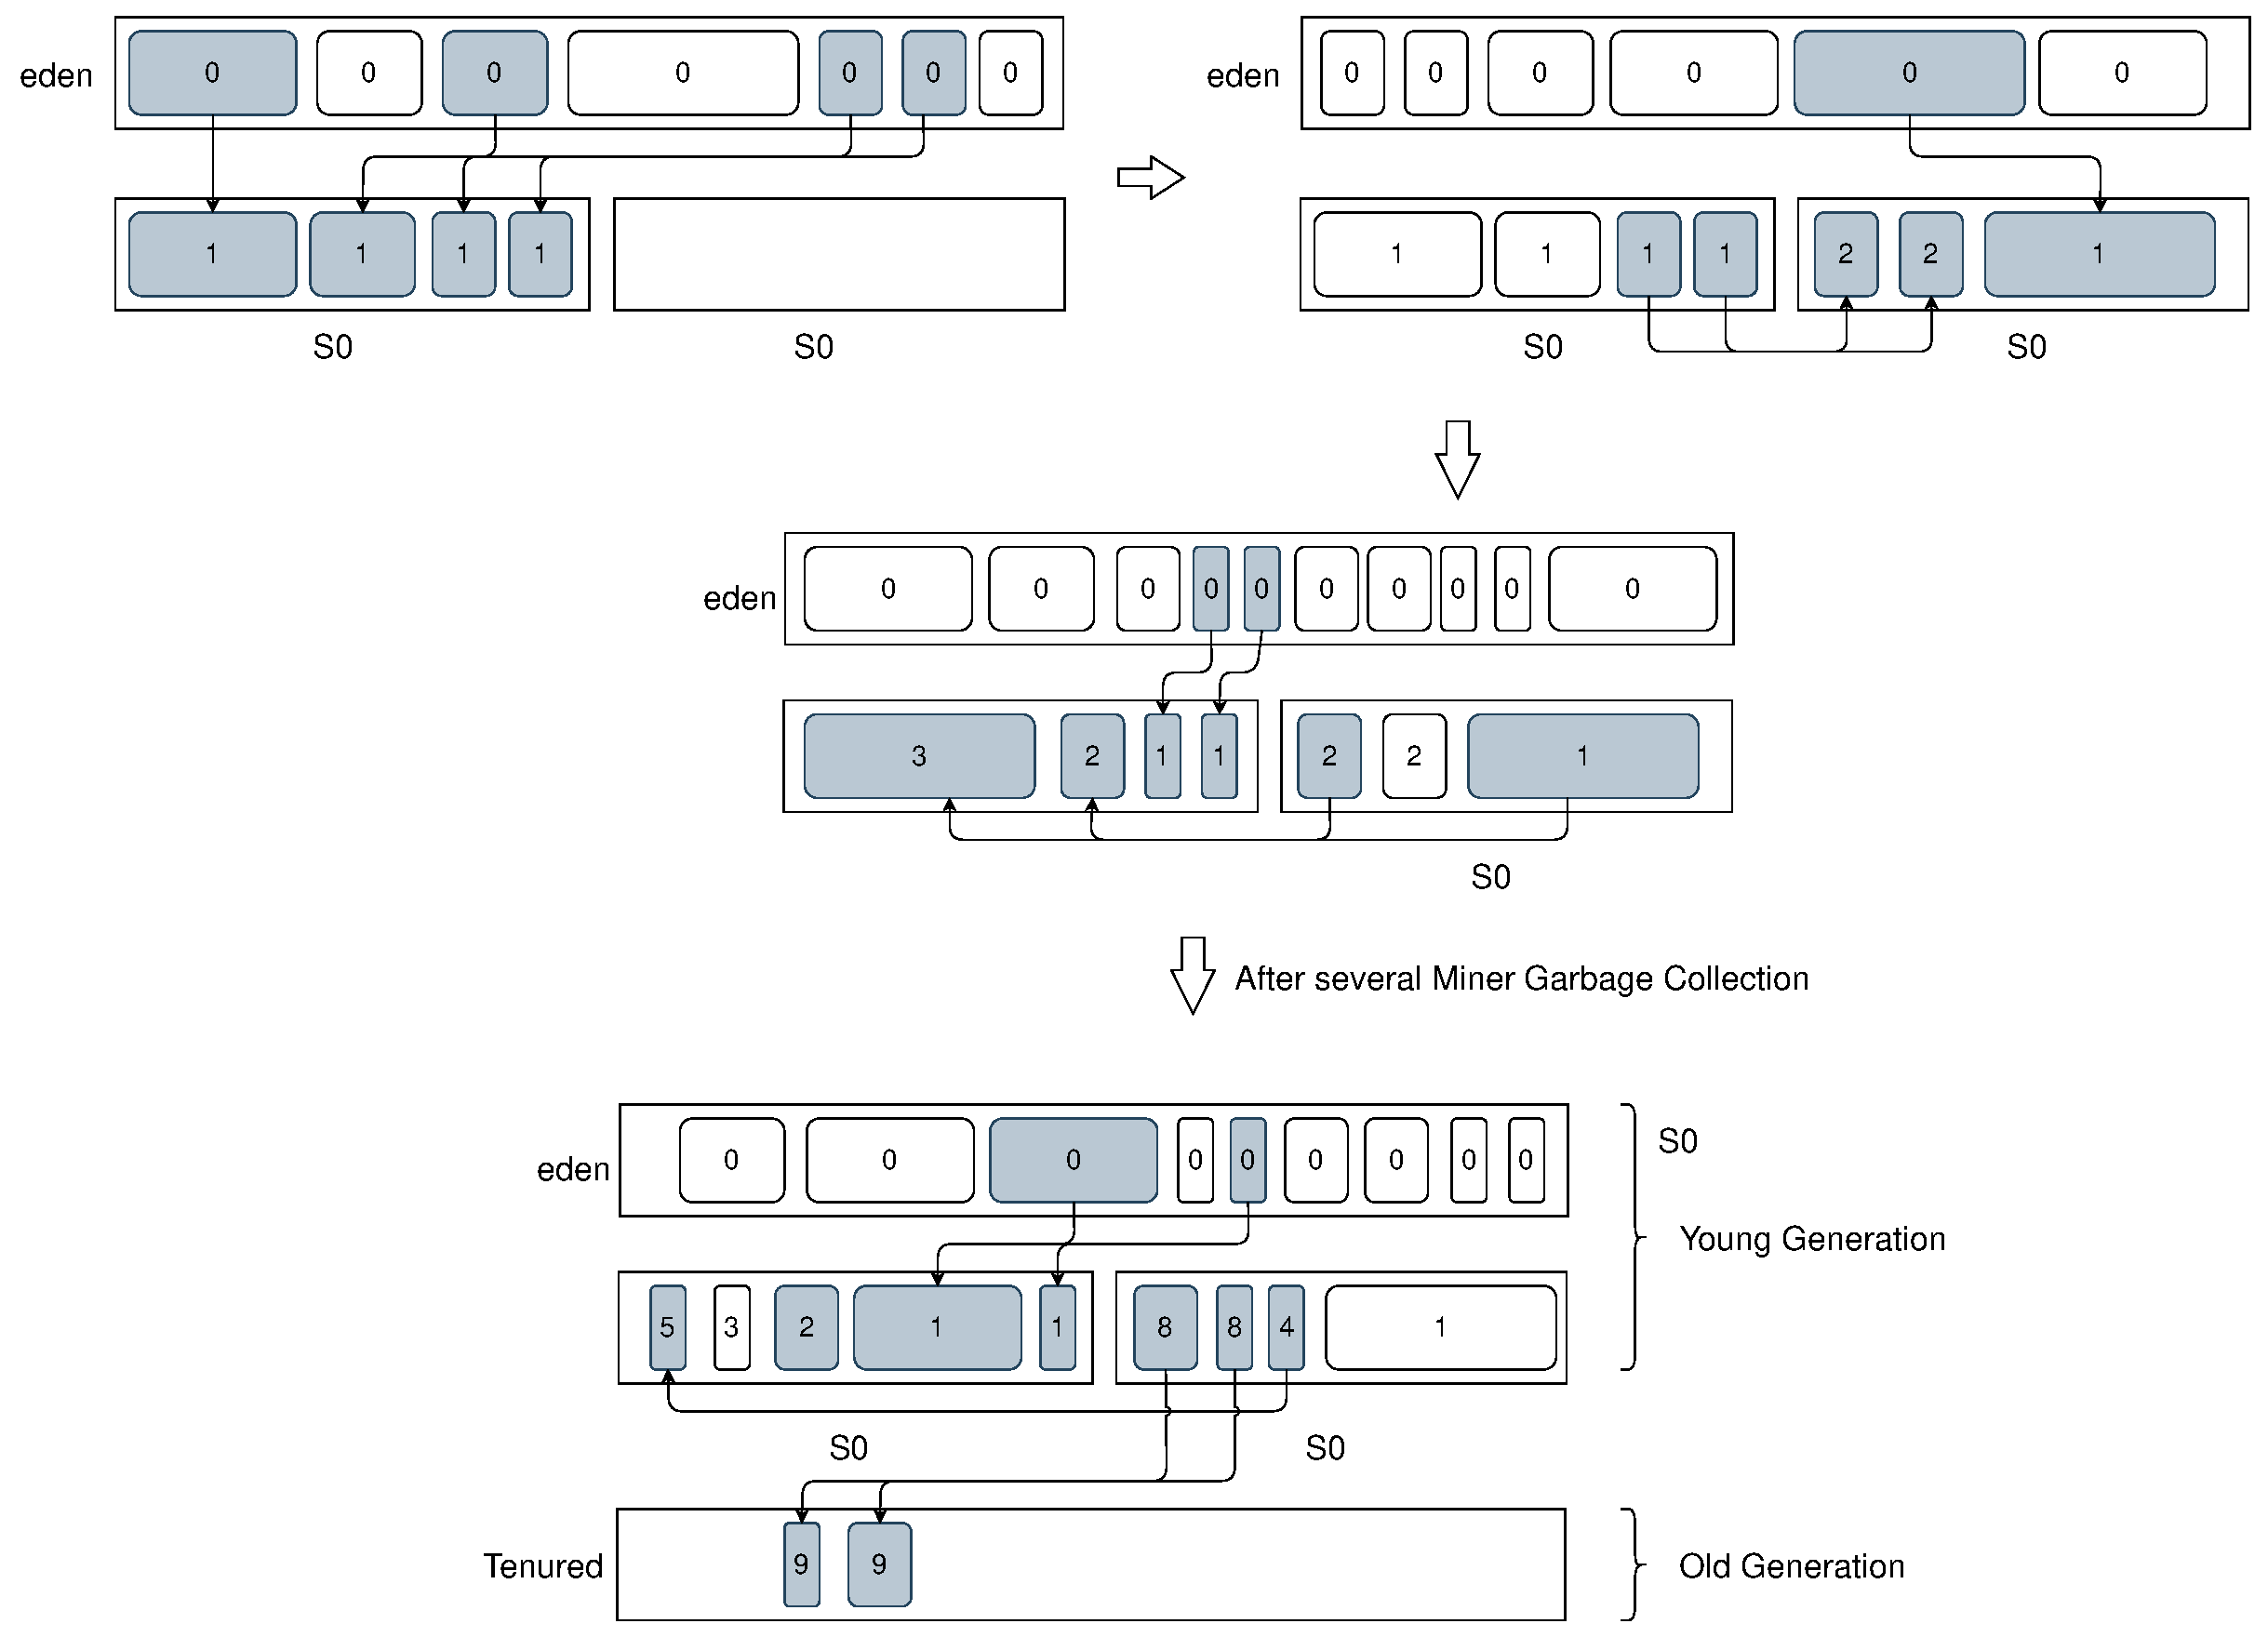
\includegraphics[width=15cm]{java_gc.eps}
    \caption{Java Garbage Collection}
    \label{fig:javagc}
\end{figure}


\subsection{Garbage Collection Tuning}
There are many different ways that one can improve the performance of GC in Java. One of these is for example avoiding pointer-based data structures, such as HashMap and LinkedList. 
These objects have a "wrapper" object for each entry so that number of object tends to be larger than when when an array is used.

Caching serialized object in memory also reduce number of object and memory usage since the set of objects become a byte or binary array. 
Spark SQL applications use DataFrames\cite{DBLP:conf/sigmod/ArmbrustXLHLBMK15}, 
whose intermediate data are managed by an optimized memory manager named Tungsten.
Tungsten stores the intermediate data in a serialized binary form and performs aggregation functions directly on he serialized objects.
Therefore, the number of Java objects in memory is reduced and it reduces the DC frequency and object marking/sweeping. 

In addition, developers can allocate data off-heap of JVM to avoid tracking by GC. 
Facade\cite{DBLP:conf/asplos/NguyenWBFHX15} proposed a compiler and runtime system to bound the number of in-memory data objects, through storing data in an off-heap region and 
manipulating the data with control interfaces.

Although these memory management solution for GC help developer improve performance of Spark applications, 
the effort to discover the best GC tuning afflicts developers.

\section{Application to System Language}
\label{sec:history}
Considered overhead produced by Memory Management in JVM, use of system language for development of Big Data tool can be one of solutions rather than application language, such as Java and Scala. 
System languages, such as C and C++, are languages that give developer total control over the hardware and de/allocation of memory without GC. 
These features enable program written in system languages to optimized performance taking full advantage of hardware. 

To take example, one can build Big Data tool with C++. C++ is one of the most popular system languages which has Object-oriented features. 
C++ has functions which provide control over memory to developers. In another word, it is responsibility for one to manage memory properly and safely. 
The functions, malloc() and free(), take roll for memory allocation and deallocation in respectively. The manual memory de/allocation may cause several problems and require developers 
attention to the problems with significant effort for debugging and testing. Here, we explain two of the most common problems regarding to memory management in existing system languages.

Dangling pointer or reference is a pointer or reference pointing to object that no longer exists. The situation of dangling pointer happens 
because of deallocation of memory without modification of value of the pointer. 
If the memory region is reallocated for other object and the dangling pointer tries to access the original object, the unpredictable behavior may result. 

Memory leak occurs when memory is allocated and no longer referenced so that the object in the memory location cannot be reached and released.
This is result of dereferencing object without deallocation. Memory leak consumes more memory than necessary by making unreachable location.

Some solutions are established to address these problems. Actually GC is a high-level solution that guarantees memory safety. 
C++ has a different solution called Resource Acquisition is Initialization (RAII). In RAII, objects can live within the scope where they are created. 
The memory is released when the object goes out of scope. This solution is more predictable and deterministic than GC. 
However, it is problematic When we need the object out of the scope, returning a value from a function. 
There are several ways to go around this problems, such as smart pointers, copy constructors, and move semantics. 
Nevertheless, these non-orthogonal concepts makes code in disorganize and leads to error prone implementation. 


\section{Rust Memory Management}
\label{sec:history}
Rust is a system programming language which provides memory safety without runtime checking like GC and necessity of explicit memory de/allocation. 
To ensure memory safety, Rust provides restrictive coding patterns and checks lifetime of value and memory safety at compile-time.
The restrictive patterns also enables a developer to write fearless concurrent code that is free of data races.
Main concepts of Memory Management in Rust are ownership, move, and borrowing.

\subsection{Ownership}
In ownership feature or Rust, each value has a variable called owner.
This owner has information about the value, such as location in memory, length and capacity of the value. 
For example, the object representation of Vec$<$i32$>$ is shown in Figure~\ref{fig:rustvec}. The upper boxes represent owner variable in stack frame. 
The lower boxes represent contiguous memory allocated to store i32. Its capacity is specified 10, but 7 values of i32 are stored. 
Therefore, there are still spaces to store 3 values of i32 without reallocation of memory. This owner can live on the scope associated with its lifetime.
When the owner is dropped, the value will be dropped too. This feature is similar to how RAII in C++ works. 
However, acquisition of owner out of the scope where it was constructed is available in Rust with the concept of move. 

\begin{figure}[htb]
    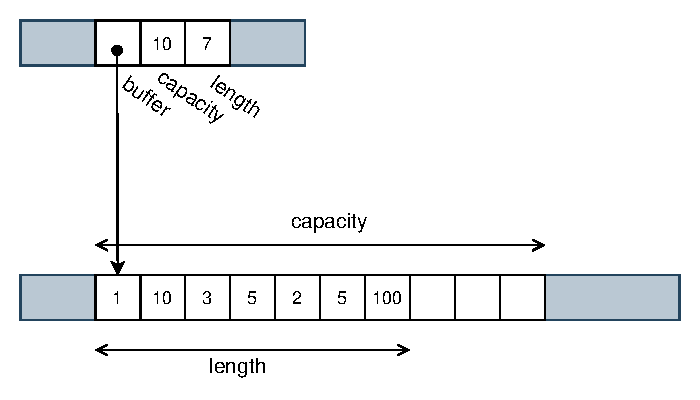
\includegraphics[width=15cm]{rust_vec.eps}
    \caption{Representation of Rust Vec$<$i32$>$}
    \label{fig:rustvec}
\end{figure}



\subsection{Move}
In Rust, for most types. operations like assigning a value to a variable, passing it to a function, or returning it from a function do not copy the value: they move it. 
With move, a value can be transferred from one owner to another. The previous variable does not have ownership of the value; it is moved to a newly assigned variable. 
To understand how this assignment implementation is unique from other programing languages, Python, C++, and Rust code example of assigning list or vector of strings are shown in Figure. 
For example, a value is instantiated in a function. 
When it is returned to a new variable, the ownership of value is moved to the new variable. In Rust, one do not have to explicitly deallocate memory, 
because ownership of value is passed among variables across scope using move and eventually goes out of scope deallocating memory of the value.

\subsection{Borrowing}
Borrowing lets code use a value temporarily without affecting its ownership so that it reduces unnecessary movement of ownership. 
One use case is when value is used in function and needed to be passed to the argument. If the argument takes ownership and the function does not return the value, 
the ownership of value goes out of scope and the memory is deallocated. One can pass reference of the value to the argument instead of owner. 
The reference goes out of scope, but ownership remains the same. 



